\documentclass{beamer}

%\usefonttheme[onlymath]{serif} %%%%%%%%%

\usetheme{NRLpresentation}



%\titlegraphic{\includegraphics[width=0.9\textwidth]{$HOME/Documents/TAVEX/gmt/TAVEX-overview-3}}% optional


\usepackage{cite}
\usepackage{amsmath,amssymb,amsfonts}
\usepackage{algorithmic}
\usepackage{graphicx}
\usepackage{textcomp}
\usepackage{bm}
\usepackage{upgreek}

\usepackage[retainorgcmds]{IEEEtrantools}

%\usepackage{hyperref}


%\graphicspath{ {C:/Users/Paul/Documents/PhD/Dissertation/Documentation/Figures/} }
\graphicspath{ {../Figures/} }


\DeclareMathOperator*{\argmin}{arg\,min}
\DeclareMathOperator*{\argmax}{arg\,max}

\DeclareMathOperator{\xrm}{\mathrm{x}}
\DeclareMathOperator{\Xrm}{\mathrm{X}}
\DeclareMathOperator{\yrm}{\mathrm{y}}
\DeclareMathOperator{\Yrm}{\mathrm{Y}}
\DeclareMathOperator{\Drm}{\mathrm{D}}
\DeclareMathOperator{\nrm}{\mathrm{n}}
\DeclareMathOperator{\nbarrm}{\bar{\mathrm{n}}}
\DeclareMathOperator{\zrm}{\mathrm{z}}

\DeclareMathOperator{\Prm}{\mathrm{P}}
\DeclareMathOperator{\prm}{\mathrm{p}}
\DeclareMathOperator{\Erm}{\mathrm{E}}
\DeclareMathOperator{\Crm}{\mathrm{C}}

\DeclareMathOperator{\Xcal}{\mathcal{X}}
\DeclareMathOperator{\Ycal}{\mathcal{Y}}
\DeclareMathOperator{\Dcal}{\mathcal{D}}
\DeclareMathOperator{\Ncal}{\mathcal{N}}
\DeclareMathOperator{\Zcal}{\mathcal{Z}}
\DeclareMathOperator{\Hcal}{\mathcal{H}}
\DeclareMathOperator{\Fcal}{\mathcal{F}}
\DeclareMathOperator{\Rcal}{\mathcal{R}}
\DeclareMathOperator{\Mcal}{\mathcal{M}}
\DeclareMathOperator{\Scal}{\mathcal{S}}
\DeclareMathOperator{\Pcal}{\mathcal{P}}
\DeclareMathOperator{\Lcal}{\mathcal{L}}

\DeclareMathOperator{\Rbb}{\mathbb{R}}
\DeclareMathOperator{\Nbb}{\mathbb{N}}
\DeclareMathOperator{\Zbb}{\mathbb{Z}}

\DeclareMathOperator{\Dir}{\mathrm{Dir}}
\DeclareMathOperator{\DM}{\mathrm{DM}}
\DeclareMathOperator{\Multi}{\mathrm{Multi}}
\DeclareMathOperator{\DP}{\mathrm{DP}}
\DeclareMathOperator{\DMP}{\mathrm{DMP}}






\title{Bayesian Learning for Classification using a Uniform Dirichlet Prior}
%\subtitle{Work Supported by the U.S. Office of Naval Research}% optional

\author[Rademacher \& Doroslova\v{c}ki]{Paul Rademacher\inst{1} \and Milo\v{s} Doroslova\v{c}ki\inst{2}}
\institute[NRL,~GWU] 
{
  \inst{1}
  U.S. Naval Research Laboratory\\Radar Division
  \and
  \inst{2}
  The George Washington University\\Department of Electrical and Computer Engineering
}


\date{November 13, 2019}


%\NRLcredit{Work Supported by the U.S. Office of Naval Research}% optional
%\NRLmark{FOR OFFICIAL USE ONLY}% optional
%\NRLpatents{Example Patents\\7,749,438 and 7,754,145}% optional



\begin{document}


\begin{frame}
\titlepage
\end{frame}


\begin{frame}
\frametitle{Introduction}
\framesubtitle{Part I}

Bayesian approaches to machine learning attempt to make better decisions by exploiting \emph{prior knowledge} regarding the data-generating distribution:

\vspace{1em}

\begin{columns}[c]

\begin{column}{.5\linewidth}
\centering
\large \textbf{\underline{Subjective}} \normalsize

\end{column}

\begin{column}{.5\linewidth}
\centering
\large \textbf{\underline{Non-Informative}} \normalsize

\end{column}

\end{columns}

\begin{columns}[T]

\begin{column}{.5\linewidth}

\begin{itemize}
\item If the prior is localized around the true data-generating model, low-risk decisions can be made even with limited training data
\item Priors that assign low weighting to the true model may not be able to realize satisfactory performance 
\end{itemize}


\end{column}

\begin{column}{.5\linewidth}

\begin{itemize}
\item Learners designed with approximately uniform priors will not perform as well as those made with well-selected subjective priors
\item Avoid high risk inherent to learners made by mismatched subjective priors
\end{itemize}



\end{column}

\end{columns}

\end{frame}




\begin{frame}
\frametitle{Introduction}
\framesubtitle{Part II}

\begin{itemize}
\item Often, priors are termed non-informative as long as they are approximately uniform over their support. For example, Gaussian conditional with mean linear in vector prior
\vspace{0.5em}
\item The uniform Dirichlet distribution is unique in that it has \underline{full support} over the space of data-generating distributions and is thus truly non-informative
\vspace{0.5em}
\item Additionally, it is a \emph{conjugate prior} for independent, identically distributed observations and leads to a closed-form model posterior distribution

\end{itemize}

PGR: MOVE DIR POINTS TO LATER SECTION?

\end{frame}



\section{Setup}


\begin{frame}
\frametitle{Data Model}

\begin{description}
\item[Observable random element:] $\xrm \in \Xcal$
\item[Unobservable random element:] $\yrm \in \Ycal$
\item[Observable training data:] $\Drm \in \Dcal = \{\Ycal \times \Xcal\}^N$
\end{description}

\vspace{0.5em}

Independently, identically distributed according to an \underline{unknown} probability mass function (PMF) 
\begin{equation*}
\theta \in \Theta = \left\{ \theta \in {\Rbb_{\geq 0}}^{\Ycal \times \Xcal}: \sum_{y \in \Ycal} \sum_{x \in \Xcal} \theta(y,x) = 1 \right\} \ ,
\end{equation*}
such that $\Prm_{\yrm,\xrm | \uptheta}(y,x | \theta) = \Prm_{\Drm_n | \uptheta}(y,x | \theta) = \theta(y,x)$.

\vspace{1em}
\textit{Alternate Representation}: $\uptheta \equiv \big( \uptheta',\tilde{\uptheta} \big)$
\begin{itemize}
\item Marginal model $\uptheta' \equiv \sum_{y \in \Ycal} \uptheta(y,\cdot)$ over the set $\Xcal$ 
\item Conditional models $\tilde{\uptheta}(x) \equiv \uptheta(\cdot,x) / \uptheta'(x)$ over the set $\Ycal$
\end{itemize}
%\begin{itemize}
%\item Marginal model $\uptheta' \equiv \sum_{y \in \Ycal} \uptheta(y,\cdot)$ over the set $\Xcal$ 
%\item Conditional models $\tilde{\uptheta}(x) \equiv \uptheta(\cdot,x) / \uptheta'(x)$ over the set $\Ycal$
%\end{itemize}


\end{frame}



\begin{frame}
\frametitle{Sufficient Statistic}

Dependency on $\Drm$ of conditional training data PMF,
\begin{IEEEeqnarray}{C}
\Prm_{\Drm | \uptheta}(D | \theta) = \prod_{y \in \Ycal} \prod_{x \in \Xcal} \theta(y,x)^{\bar{N}(y,x;D)} \nonumber \;,
\end{IEEEeqnarray}
is expressed via $\bar{N}(y,x;D) = \sum_{n=1}^N \delta\big[ (y,x),D_n \big]$, with range $\bar{\Ncal} = \left\{ \bar{n} \in {\Zbb_{\geq 0}}^{\Ycal \times \Xcal}: \sum_{y \in \Ycal} \sum_{x \in \Xcal} \bar{n}(y,x) = N \right\}$

\vspace{1em}
 
\begin{itemize}
\item Empirical count $\bar{N}(\Drm)$ is a \emph{sufficient statistic} for the model $\uptheta$
\item $|\bar{\Ncal}| = \binom{N+|\Ycal||\Xcal|-1}{|\Ycal||\Xcal|-1} \leq |\Dcal|$  $\quad \longrightarrow \quad$ \underline{Efficient Transform} 
%\item[$\Rightarrow$] Express distributions using new random process $\nbarrm \equiv \bar{N}(\Drm) \in \bar{\Ncal}$
\end{itemize}
\Large
\begin{equation*} 
\Downarrow \quad \Downarrow
\end{equation*}
\normalsize
\textbf{Express distributions using new random process $\nbarrm \equiv \bar{N}(\Drm) \in \bar{\Ncal}$}

\end{frame}



\begin{frame}
\frametitle{Objective}

User-selected function $\Lcal: \Ycal \times \Ycal \mapsto \Rbb_{\geq 0}$. Most commonly selected for classification is the 0--1 loss:
\begin{equation*}
\Lcal(h,y) = 1 - \delta[h,y]
\end{equation*}


\begin{alertblock}{Design}
Decision function $f: \bar{\Ncal} \mapsto \Ycal^{\Xcal}$

Minimizes the conditional expected loss, or conditional ``risk'',
\begin{IEEEeqnarray}{L} \label{eq:risk_cond}
\Rcal_{\Theta}(f ; \uptheta) = \Erm_{\xrm,\nbarrm | \uptheta} \bigg[ \Erm_{\yrm | \xrm,\uptheta} \Big[ \Lcal\big( f(\xrm;\nbarrm),\yrm \big) \Big] \bigg] \nonumber \\
= 1 - \Erm_{\xrm,\nbarrm | \uptheta} \Big[ \Prm_{\yrm | \xrm,\uptheta}\big( f(\xrm;\nbarrm) \big) \Big] \nonumber
\end{IEEEeqnarray}

\end{alertblock}


\end{frame}



\begin{frame}
\frametitle{Clairvoyant Hypothesis and Risk}

\begin{columns}[c]
%\begin{columns}[T, totalwidth=\textwidth]

\begin{column}{.5\linewidth}

The ``clairvoyant'' classifier $f_{\uptheta}: \Theta \mapsto \Ycal^{\Xcal}$ is maximum \textit{a posteriori} (MAP): 
\begin{IEEEeqnarray}{rCl} \label{eq:f_clv_01}
f_{\Theta}(\xrm;\uptheta) & = & \argmin_{h \in \Ycal} \Erm_{\yrm | \xrm,\uptheta} \left[ 1 - \delta[h,y] \right] \nonumber \\
& = & \argmax_{y \in \Ycal} \tilde{\uptheta}(y;\xrm) \nonumber
\end{IEEEeqnarray}
\Large
\begin{equation*} 
\Downarrow \quad \Downarrow
\end{equation*}
\normalsize
\begin{IEEEeqnarray}{rCl}
\Rcal_{\Theta}^*(\uptheta) & = & 1 - \sum_{x \in \Xcal} \uptheta'(x) \max_{y \in \Ycal} \tilde{\uptheta}(y;x) \nonumber 
\end{IEEEeqnarray}

\end{column}

\begin{column}{.5\linewidth}

\begin{figure}
\centering
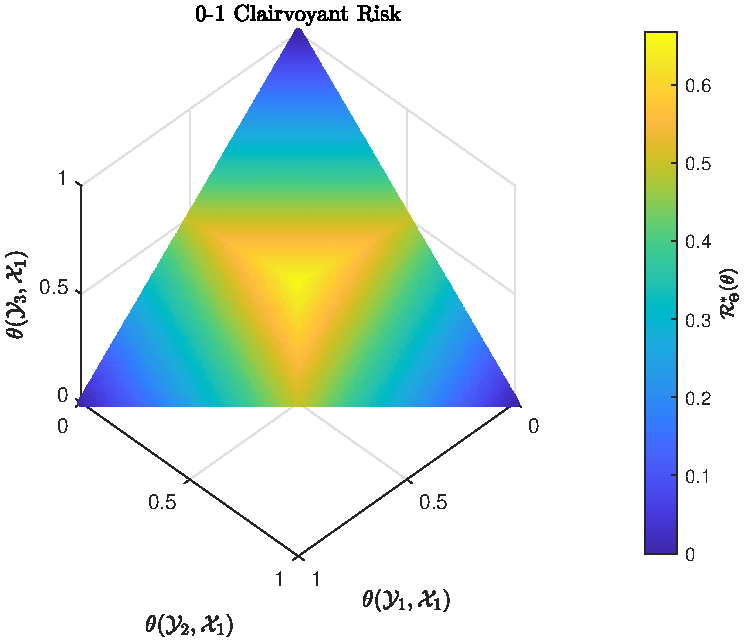
\includegraphics[width=1\linewidth]{Risk_clv_01.pdf}
%\caption{Model Posterior for an example training set $\nbarrm$}
\label{fig:Risk_clv_01}
\end{figure}

\end{column}

\end{columns}

\end{frame}



\begin{frame}
\frametitle{Bayesian Inference}

\large
\begin{equation*} 
\Downarrow \quad \Downarrow \quad \textbf{\textit{Model Unknown. Select Prior }} \bm{\mathrm{p}_\uptheta} \quad \Downarrow \quad \Downarrow 
\end{equation*}
\normalsize
\begin{IEEEeqnarray}{C} \label{eq:risk}
\Rcal(f) = \Erm_{\uptheta}\big[ \Rcal_{\Theta}(f ; \uptheta) \big] = 1 - \Erm_{\xrm,\nbarrm}\Big[ \Prm_{\yrm | \xrm,\nbarrm} \big( f(\xrm;\nbarrm) \big) \Big] \nonumber
\end{IEEEeqnarray}

\textbf{Optimal classifier}: Bayesian maximum \textit{a posteriori}
\begin{IEEEeqnarray*}{rCl} \label{eq:f_opt_xD}
f^*(\xrm;\nbarrm) & = & \argmax_{h \in \Ycal} \Prm_{\yrm | \xrm,\nbarrm}( h | \xrm,\nbarrm) \\
& = & \argmax_{h \in \Ycal} \Erm_{\uptheta | \xrm,\nbarrm} \Big[ \Prm_{\yrm | \xrm,\uptheta}\big( h | \xrm,\uptheta \big) \Big]
\end{IEEEeqnarray*}
%\begin{IEEEeqnarray*}{rCl} \label{eq:f_opt_xD}
%f^*(x;\bar{n}) & = & \argmax_{h \in \Ycal} \Prm_{\yrm | \xrm,\nbarrm}\big( h | x,\bar{n} \big) \\
%& = & \argmax_{h \in \Ycal} \Erm_{\uptheta | \xrm,\nbarrm} \Big[ \Prm_{\yrm | \xrm,\uptheta}\big( h | x,\uptheta \big) \Big]\big( x,\bar{n} \big)
%\end{IEEEeqnarray*}

\textbf{Minimum Bayes Probability of Error}:
\begin{equation*} \label{eq:risk_min}
\Rcal(f^*) = 1 - \Erm_{\xrm,\nbarrm} \left[ \max_{h \in \Ycal} \Prm_{\yrm | \xrm,\nbarrm}\big( h | \xrm,\nbarrm \big) \right]
\end{equation*}

\end{frame}





\section{Distributions: Prior to Predictive}

\begin{frame}
\frametitle{Dirichlet Prior PDF}

The selected PDF for the model random process $\uptheta \in \Theta$ is Dirichlet with parameters $\alpha(\cdot,\cdot) = 1$:
\begin{IEEEeqnarray*}{rCl}
\prm_{\uptheta}(\theta) & = & \bigg[ \beta(\alpha)^{-1} \prod_{y \in \Ycal} \prod_{x \in \Xcal} \theta(y,x)^{\alpha(y,x) - 1} \bigg]_{\alpha(\cdot,\cdot) = 1} \\
& = & \big( |\Ycal||\Xcal|-1 \big)!  
\end{IEEEeqnarray*}
is uniform over $\Theta$. 

For convenience, the Dirichlet concentration parameter is defined as $\alpha_0 \equiv \sum_{y \in \Ycal} \sum_{x \in \Xcal} \alpha(y,x)$. The mean function of the model is 
\begin{equation*}
\mu_{\uptheta}(y,x) = \frac{\alpha(y,x)}{\alpha_0}\bigg|_{\alpha(\cdot,\cdot) = 1} = \big( |\Ycal||\Xcal| \big)^{-1} \;.
\end{equation*}

\end{frame}


\begin{frame}
\frametitle{Dirichlet Prior PDF}

%Marginal model $\uptheta' \equiv \sum_{y \in \Ycal} \uptheta(y,\cdot)$ over the set $\Xcal$ 
%
%Conditional models $\tilde{\uptheta}(x) \equiv \uptheta(\cdot,x) / \uptheta'(x), \; \forall x \in \Xcal$ over the set $\Ycal$

Conditional PDF of $\tilde{\uptheta}$ given $\uptheta'$ is
\begin{IEEEeqnarray*}{rCl}
\prm_{\tilde{\uptheta} | \uptheta'}\big( \tilde{\theta} | \theta' \big) & = & \prm_{\tilde{\uptheta}}\big( \tilde{\theta} \big) = \prod_{x \in \Xcal} \Bigg[ \beta\big( \alpha(\cdot,x) \big)^{-1} \prod_{y \in \Ycal} \tilde{\theta}(y;x)^{\alpha(y,x)-1} \Bigg]_{\alpha(\cdot,x) = 1} \\
& = & \Big[ \big( |\Ycal|-1 \big)! \Big]^{|\Xcal|}
\end{IEEEeqnarray*}
a product of Dirichlet distributions defined for $\tilde{\theta} \in \tilde{\Theta}^{\Xcal}$, where $\tilde{\Theta} = \left\{ p \in {\Rbb_{\geq 0}}^{\Ycal} : \sum_{y \in \Ycal} p(y) = 1 \right\}$. 

Note that $\Prm_{\yrm | \xrm,\uptheta}(y | x,\theta) \equiv \tilde{\theta}(y;x)$ compactly notates the true predictive distribution. 

\end{frame}


\begin{frame}
\frametitle{Dirichlet Prior PDF}

\begin{figure}
\centering
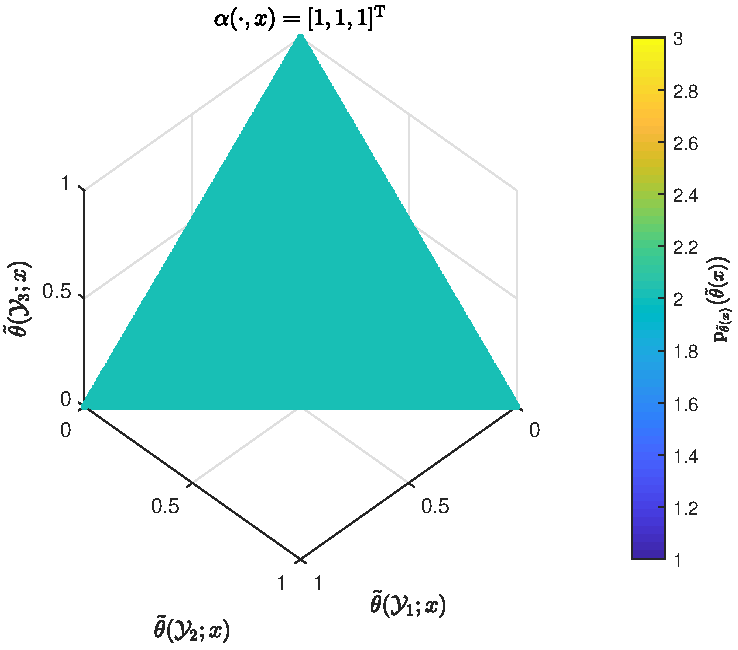
\includegraphics[width=1\linewidth]{P_theta_uniform_tilde.pdf}
\caption{Uniform model prior PDF, $|\Ycal| = 3$, $|\Xcal| = 1$}
\label{fig:P_theta_uniform}
\end{figure}

\end{frame}








\begin{frame}
\frametitle{Sufficient Statistic PMF}

Data statistic conditioned on model: $\nbarrm | \uptheta \sim \Multi(N,\uptheta)$

Data statistic marginal is a Dirichlet-Multinomial distribution parameterized by $\alpha(\cdot,\cdot) = 1$,
\begin{IEEEeqnarray}{rCl}
\Prm_{\nbarrm}(\bar{n}) & = & \Mcal(\bar{n}) \beta(\alpha)^{-1} \beta(\alpha + \bar{n}) \big|_{\alpha(\cdot,\cdot) = 1} \\
& = & |\bar{\Ncal}|^{-1} = \binom{N+|\Ycal||\Xcal|-1}{|\Ycal||\Xcal|-1}^{-1} \nonumber \;,
\end{IEEEeqnarray}
which is uniform over the set $\bar{\Ncal}$. 

PGR: move to risk assessment section?

\end{frame}


\begin{frame}
\frametitle{Sufficient Statistic PMF}

\begin{figure}
\centering
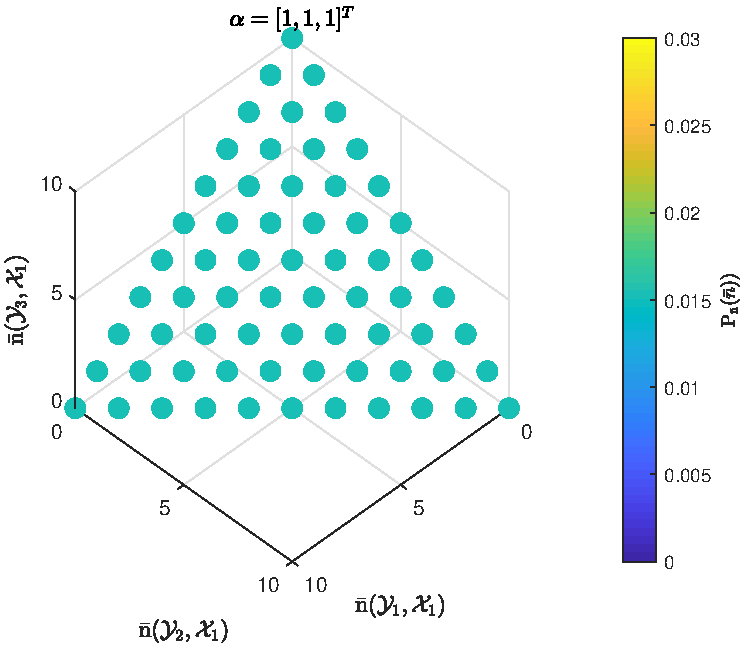
\includegraphics[width=1\linewidth]{P_nbar_uni.pdf}
%%\caption{Uniform model prior PDF, $|\Ycal| = 3$, $|\Xcal| = 1$}
%%\label{fig:P_theta_uniform}
\end{figure}

\end{frame}



\begin{frame}
\frametitle{Model Posterior PDF}

$\Prm_{\yrm | \xrm,\nbarrm} = \Erm_{\uptheta | \xrm,\nbarrm}\big[ \Prm_{\yrm | \xrm,\uptheta} \big] = \mu_{\tilde{\uptheta}(\xrm) | \xrm,\nbarrm}$, the conditional expectation of the predictive model $\tilde{\uptheta}(\xrm)$

\textbf{Dirichlet prior}:since the conditional models $\tilde{\uptheta}(x)$ are independent of the marginal model $\uptheta'$, they are also conditionally independent of $\xrm$ given the statistic $\nbarrm$

\begin{IEEEeqnarray}{L}
\prm_{\tilde{\uptheta} | \xrm,\nbarrm}\big( \tilde{\theta} | x,\bar{n} \big) = \prm_{\tilde{\uptheta} | \nbarrm}\big( \tilde{\theta} | \bar{n} \big) \\
= \prod_{x' \in \Xcal} \left[ \beta \big( \alpha(\cdot,x') + \bar{n}(\cdot,x') \big)^{-1} \prod_{y \in \Ycal} \tilde{\uptheta}(y;x')^{\alpha(y,x') + \bar{n}(y,x') - 1} \right]_{\alpha(\cdot,x') = 1} \nonumber \\
= \prod_{x' \in \Xcal} \left[ \left( \sum_{y \in \Ycal} \bar{n}(y,x') + |\Ycal|-1 \right)! \prod_{y \in \Ycal} \frac{\tilde{\theta}(y,x')^{\bar{n}(y,x')}}{\big(\sum_{y \in \Ycal} \bar{n}(y,x')\big)!} \right] \nonumber
\end{IEEEeqnarray}
%\begin{IEEEeqnarray}{rCl}
%\prm_{\uptheta | \Drm}(\theta | D) & = & \big(N+|\Ycal|-1\big)! \prod_{y \in \Ycal} \frac{\tilde{\theta}(y,x')^{\bar{n}(y,x')}}{\big(\sum_{y \in \Ycal} \bar{n}(y,x')\big)!} \nonumber \;.
%\end{IEEEeqnarray}

each model $\tilde{\uptheta}(x)$ dependent solely on the sufficient statistic elements $\nbarrm(\cdot,x)$.

\end{frame}



\begin{frame}
\frametitle{Model Posterior PDF}

\begin{columns}[T]
%\begin{columns}[T, totalwidth=\textwidth]

\begin{column}{.5\linewidth}

The concentration parameters increase proportionately with the volume of training data. Thus as each $n'(x) \to \infty$, the posteriors converges to $\prm_{\tilde{\uptheta}(x) | \nbarrm(\cdot,x)}\big(\tilde{\theta}(x) | \bar{n}(\cdot,x) \big) \to \delta\big( \tilde{\theta}(x) - \bar{n}(\cdot,x) / \sum_y \bar{n}(y,x) \big)$ and the conditional models are identified.

PGR: full support!

\end{column}

\begin{column}{.5\linewidth}

\begin{figure}
\centering
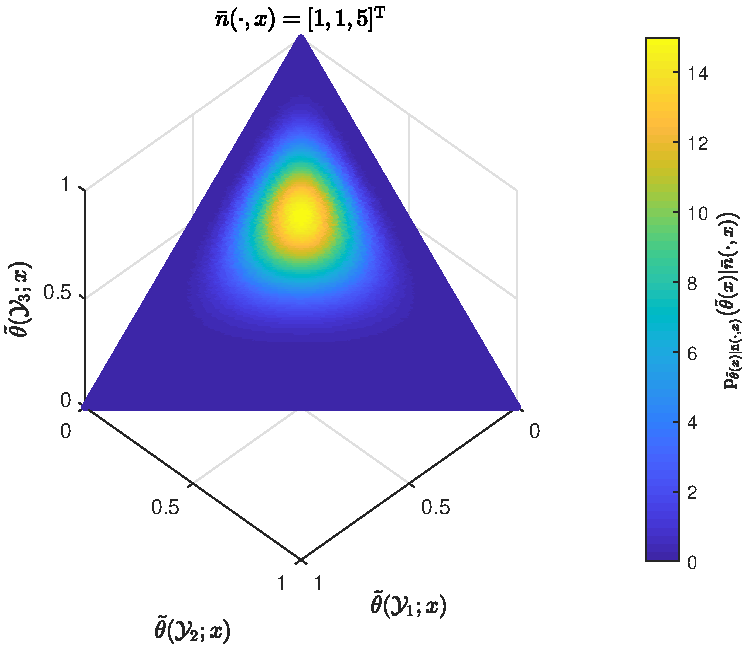
\includegraphics[width=1\linewidth]{P_theta_post_uni_tilde.pdf}
%\caption{Model Posterior for an example training set $\nbarrm$}
\label{fig:P_theta_post_uni}
\end{figure}

\end{column}

\end{columns}

\end{frame}


\begin{frame}
\frametitle{Bayesian Predictive PMF}

\begin{IEEEeqnarray}{L} \label{P_y_xD_uniform}
\Prm_{\yrm | \xrm,\nbarrm}(y | x,\bar{n}) = \mu_{\tilde{\uptheta}(\xrm) | \xrm,\nbarrm} = \mu_{\tilde{\uptheta}(\xrm) | \nbarrm(\cdot,\xrm)} = \frac{\bar{n}(y,x)+1}{\sum_{y' \in \Ycal} \bar{n}(y',x) + |\Ycal|} \nonumber \\
= \left( \frac{|\Ycal|}{\sum_{y' \in \Ycal} \bar{n}(y',x) + |\Ycal|} \right) \frac{1}{|\Ycal|} + \left( \frac{\sum_{y' \in \Ycal} \bar{n}(y',x)}{\sum_{y' \in \Ycal} \bar{n}(y',x) + |\Ycal|} \right) \frac{\bar{n}(y,x)}{\sum_{y' \in \Ycal} \bar{n}(y',x)} \nonumber 
\end{IEEEeqnarray}

The second form represents the predictive PMF as a convex combination of two conditional distributions. The first PMF $\Prm_{\yrm | \xrm} = |\Ycal|^{-1}$ is uniform and independent of the training data; the second distribution is the conditional empirical PMF. As the number of matching training data $N'(x;\Drm)$ increases relative to the number of classes $|\Ycal|$, the predictive PMF tends toward the empirical PMF.


\end{frame}





\section{Bayesian Classifier and Error Trends}


\begin{frame}
\frametitle{Bayesian Classifier and Risk}

\textbf{Optimal Hypothesis}: the \emph{conditional majority decision}
\begin{IEEEeqnarray}{rCl} 
f^*(x;\bar{n}) & = & \argmax_{h \in \Ycal} \Prm_{\yrm | \xrm,\nbarrm}\big( h | x,\bar{n} \big) = \argmax_{y \in \Ycal} \bar{n}(y,x) \nonumber
\end{IEEEeqnarray}

\textbf{Minimum Probability of Error}:
\begin{IEEEeqnarray}{L}
\Rcal^* = 1 - \Erm_{\xrm,\Drm} \left[ \max_{y \in \Ycal} \Prm_{\yrm | \xrm,\Drm}(y | \xrm,\Drm) \right] \nonumber \\
= 1 - \sum_{x \in \Xcal} \frac{\Erm_{\nbarrm} \big[ \max_{y \in \Ycal} \bar{\nrm}(y,x) \big] + 1}{|\Ycal||\Xcal| + N} \nonumber \\
= 1 - \frac{\sum_{m=1}^{|\Ycal|} \binom{|\Ycal|}{m} (-1)^{m-1} \sum_{n=0}^{\big\lfloor\frac{N}{m}\big\rfloor} \prod_{l=1}^{|\Ycal||\Xcal|-1} \Big( 1-\frac{mn}{N+l} \Big)}{|\Ycal| + N/|\Xcal|} \nonumber
\end{IEEEeqnarray}

\end{frame}


\begin{frame}
\frametitle{Bayesian Classifier and Risk}

\begin{columns}[c]

\begin{column}{.5\linewidth}

\begin{figure}
\centering
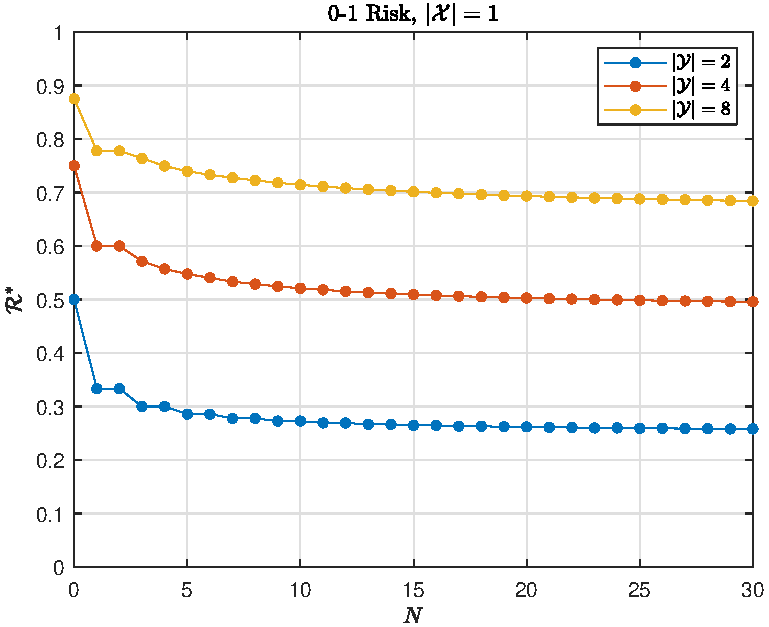
\includegraphics[width=1\linewidth]{Risk_01_uni_N_leg_My.pdf}
%\caption{Minimum 0--1 Risk for different numbers of classes}
\label{fig:Risk_01_uni_N_leg_My}
\end{figure}

\end{column}

\begin{column}{.5\linewidth}

\begin{figure}
\centering
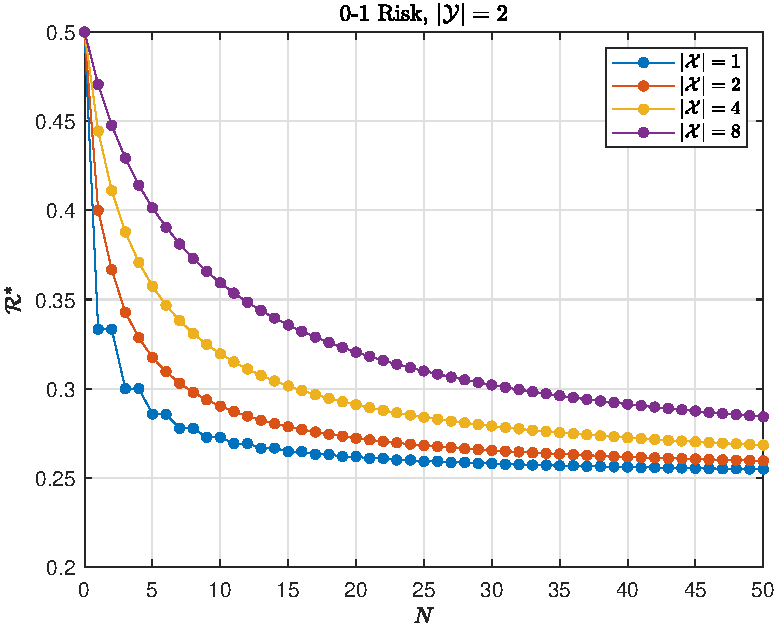
\includegraphics[width=1\linewidth]{Risk_01_uni_N_leg_Mx.pdf}
%\caption{Minimum 0--1 Risk for different numbers of possible observations}
\label{fig:Risk_01_uni_N_leg_Mx}
\end{figure}

\end{column}

\end{columns}

With a larger set of classes, accurate classification becomes more difficult; similarly, the probability of error increases with the number of possible observations $\xrm = x$

\end{frame}




\begin{frame}
\frametitle{Probability of Error Trends}

\begin{columns}[c]

\begin{column}{.5\linewidth}

\begin{itemize}
\item For binary classification, infinite training data only reduces the expected probability of error from 0.5 to 0.25
\item As $|\Ycal|$ increases, the probability of error tends to unity and any improvement due to training data becomes negligible
\end{itemize}

\begin{table}
\begin{tabular}{| c | c |}
\hline 
$N$ & $\Rcal^*$ \\
\hline \hline
$0$ & $1 - |\Ycal|^{-1}$  \\ 
\hline
$\to \infty$ & $1 - |\Ycal|^{-1} \sum_{m=1}^{|\Ycal|} m^{-1}$ \\
\hline
\end{tabular}
%\caption{}
\end{table}

\end{column}

\begin{column}{.5\linewidth}

\begin{figure}
\centering
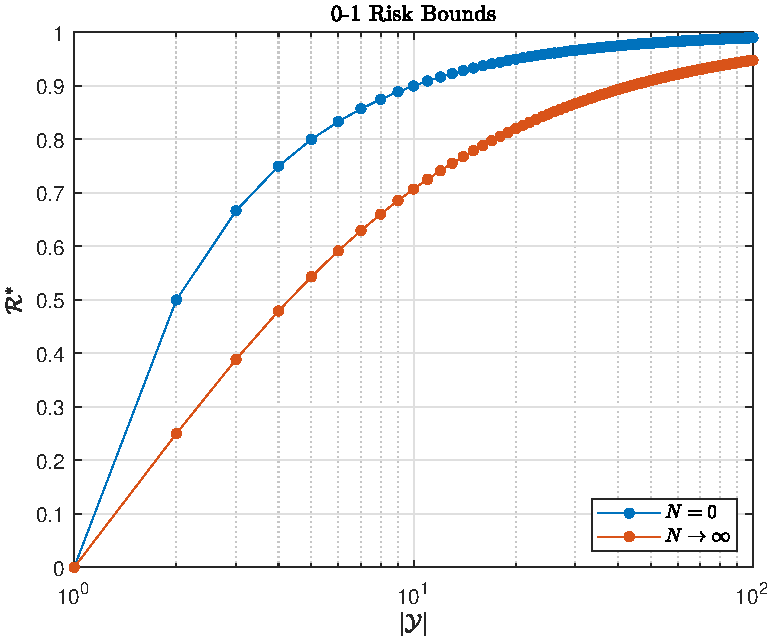
\includegraphics[width=1\linewidth]{Risk_01_uni_N_bounds.pdf}
%\caption{Minimum 0--1 Risk for zero and infinite number of training data}
\label{fig:Risk_01_uni_N_bounds}
\end{figure}

\end{column}

\end{columns}

\end{frame}


\begin{frame}
\frametitle{Bayes Risk for Subjective Classifiers}

\begin{columns}[c]

\begin{column}{.5\linewidth}

\begin{figure}
\centering
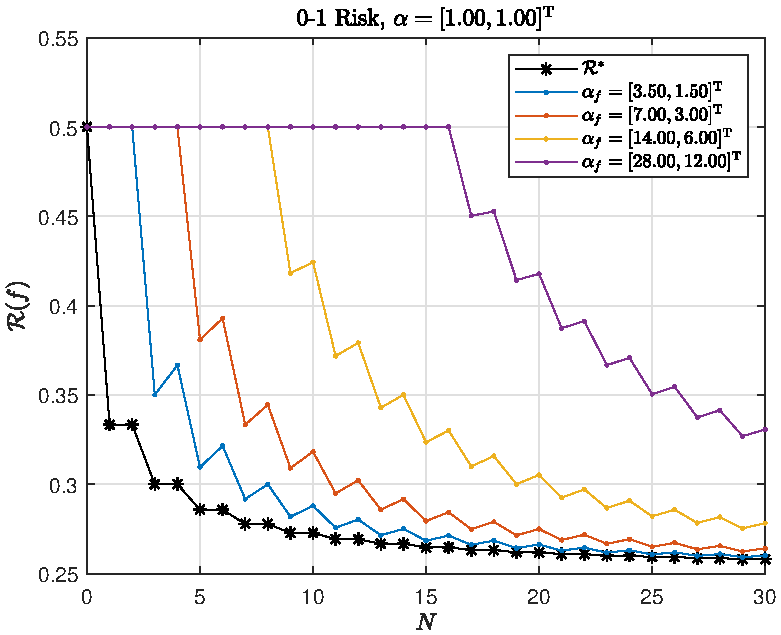
\includegraphics[width=1\linewidth]{Risk_01_Dir_N_leg_f_a0.pdf}
%\caption{}
\label{fig:Risk_01_Dir_N_leg_f_a0}
\end{figure}

\end{column}

\begin{column}{.5\linewidth}

\begin{figure}
\centering
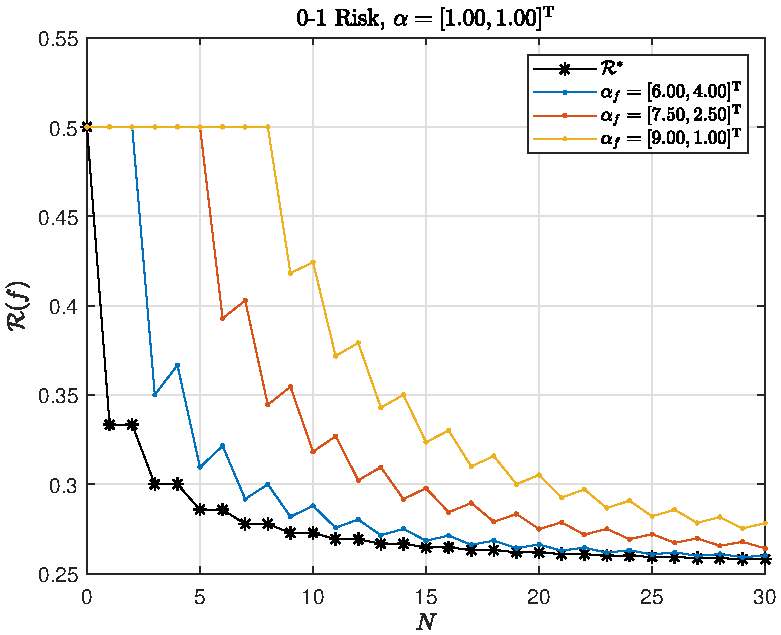
\includegraphics[width=1\linewidth]{Risk_01_Dir_N_leg_f_mu.pdf}
%\caption{}
\label{fig:Risk_01_Dir_N_leg_f_mu}
\end{figure}

\end{column}

\end{columns}

\end{frame}



\begin{frame}
\frametitle{Conditional Risk for Subjective Classifiers}

\begin{columns}[c]

\begin{column}{.5\linewidth}

\begin{figure}
\centering
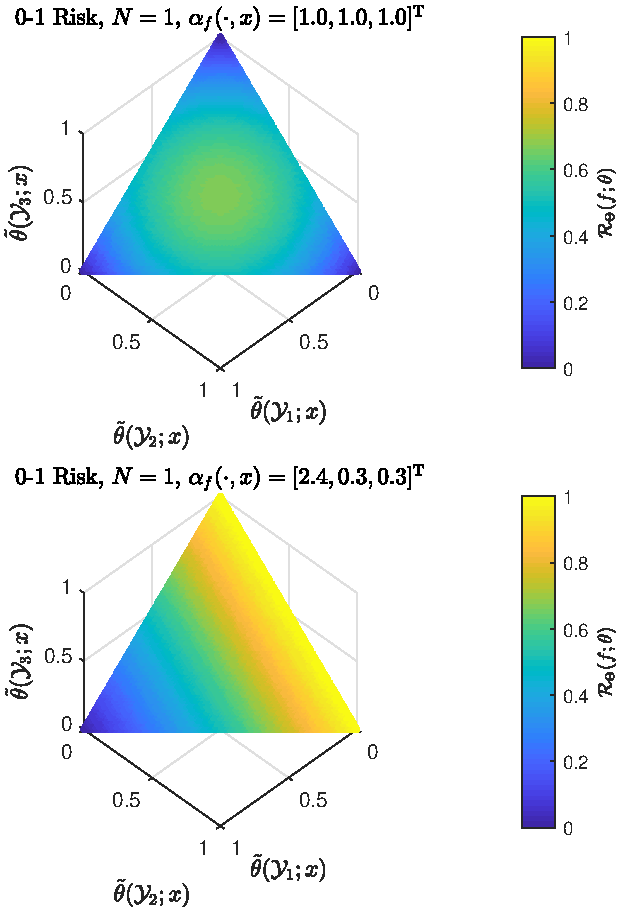
\includegraphics[width=1\linewidth]{Risk_cond_01_Dir_theta_sub_mu.pdf}
%\caption{}
\label{fig:Risk_cond_01_Dir_theta_sub_mu}
\end{figure}

\end{column}

\begin{column}{.5\linewidth}

\begin{figure}
\centering
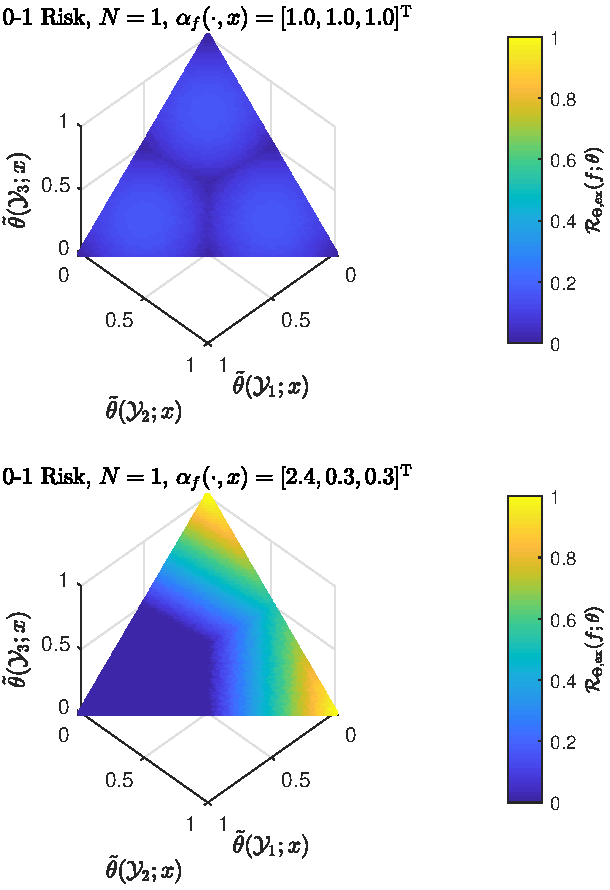
\includegraphics[width=1\linewidth]{Risk_cond_ex_01_Dir_theta_sub_mu.pdf}
%\caption{}
\label{fig:Risk_cond_ex_01_Dir_theta_sub_mu}
\end{figure}

\end{column}

\end{columns}

\end{frame}




\begin{frame}
\frametitle{Conclusions}

This work has used the non-informative uniform Dirichlet prior for Bayesian learning, discussed the Bayes predictive distribution, and applied the results to classification. The optimal majority decision learner and the minimum 0--1 risk have been analyzed. Graphical examples illustrate how the probability of error increases with the number of classes and the number of possible observations. Additionally, the asymptotic Bayes risk using infinite training data has been found and its deviation from the risk of an untrained classifier has been discussed. 

Future work will expand the results presented for a general Dirichlet prior. The effect of the subjectivity of the prior on the conditional risk \eqref{eq:risk_cond} will be of specific interest. Additionally, the work will be generalized for an infinite number of possible observations using Dirichlet processes

\end{frame}













\end{document}
